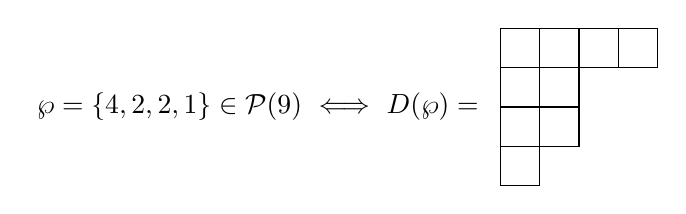
\begin{tikzpicture}[scale=0.5]
\node[anchor=east] at (-0.3,-2) {$\wp=\{4,2,2,1\}\in\mathcal{P}(9)\ \Longleftrightarrow\ D(\wp)=$};
\foreach \r/\len in {0/4, 1/2, 2/2, 3/1} {
  \foreach \c in {1,...,\len} { \draw (\c-1,-\r) rectangle (\c,-\r-1); }
}
\end{tikzpicture}
